\subsection{Observer design} \label{sec:observer}

In Section \ref{sec:rl}, we designed a controller for a simple nonlinear system assuming that the controller had \textit{full state knowledge}: that is, it had access to both the position and velocity of the box. In many practical situations, we may only be able to measure some of the system states. For example, our box may have a camera to estimate its position but not its velocity. In these cases, we need a \textit{state observer} to estimate the full state of the system for feedback control.

In this example, we will show how a contracting REN can be used to learn stable observers for dynamical systems. A common approach to designing state estimators for nonlinear systems is the \textit{Extended Kalman Filter} (EKF). In our case, we will consider observer design as a supervised learning problem. For a detailed explanation of the theory behind learning state observers, and for a similar example designing an observer for a \textit{Partial Differential Equations} (PDE), please refer to Section VIII of \cite{Revay++2021b}.

% Overview
\subsubsection{Background theory} \label{sec:observer-theory}

We briefly summarise some background theory from \cite{Revay++2021b} relevant to this example. Suppose we have a discrete-time, nonlinear dynamical system of the form
\begin{align}
    x_{t+1} &= f_d(x_t, u_t) \\
    y_t &= g_d(x_t, u_t)
\end{align}
with state vector $x_t,$ controlled inputs $u_t,$ and measured outputs $y_t.$ Our aim is to estimate the sequence $\{x_0, x_1, \ldots, x_T \}$ over some time period $[0,T]$ given only the measurements $y_t$ and inputs $u_t$ at each time step. We will use a very general form for an observer
\begin{equation}
    \hat{x}_{t+1} = f_o(\hat{x}_t, u_t, y_t)
\end{equation}
where $\hat{x}_t$ is the state estimate. A more common (but more restrictive) structure is the well-known Luenberger observer \cite{Luenberger1971}.

To estimate the true state, our observer error $(x_t - \hat{x}_t)$ must converge to zero as time progresses, or $\hat{x}_t \rightarrow x_t$ as $t \rightarrow \infty$. As outlined in \cite{Revay++2021b}, our observer only has to satisfy the following two conditions to guarantee this.

\begin{enumerate}
    \item The observer must be a contracting system (Sec. \ref{sec:robustness-contraction}).
    \item The observer must satisfy a ``correctness'' condition which says that, given perfect knowledge of the state, measurements, and inputs, the observer can exactly predict the next state. Mathematically, we write this as
    \begin{equation}
        f_o(x_t,u_t,y_t) = f_d(x_t,u_t)
    \end{equation}
    where $y_t = g_d(x_t,u_t)$. Note the use of $x_t$ not $\hat{x}_t$. It turns out that if the correctness condition is only approximately satisfied such that $|f_o(x_t,u_t,y_t) - f_d(x_t,u_t)| < \rho$ for some small number $\rho\in\mathbb{R}$, then the observer error will still be bounded. See Appendix E of \cite{Revay++2021b} for details.
\end{enumerate}

The first condition, contraction, is already guaranteed for all REN models in \verb|RobustNeuralNetworks.jl|. Therefore, to learn a stable observer with RENs, our only requirement is to minimise the one-step-ahead prediction error to approximate the correctness condition. If we have a batch of data $z = \{x_i, u_i, y_i, \ i = 1,2,\ldots,N\},$ this corresponds to minimising the loss function
\begin{equation}
\mathcal{L}(z, \theta) = \sum_{i=1}^N |f_o(x_i,u_i,y_i) - f_d(x_i,u_i)|^2,
\end{equation}
where $\theta$ contains the learnable parameters of the REN.

% Problem setup
\subsubsection{Generate training data} \label{sec:observer-setup}

Consider the same nonlinear box system from Section \ref{sec:rl}, with the a change in setup so that we can only measure the box position. We introduce a measurement function \verb|gd()| such that $y_t = x_t$.

\begin{lstlisting}[language = Julia]
m = 1                   # Mass (kg)
k = 5                   # Spring constant (N/m)
μ = 0.5                 # Viscous damping (kg/m)
nx = 2                  # Number of states


# Continuous and discrete dynamics and measurements
f(x::Matrix,u::Matrix) = [x[2:2,:]; (u[1:1,:] - 
    k*x[1:1,:] - μ*x[2:2,:].^2)/m]
fd(x,u) = x + dt*f(x,u)
gd(x::Matrix) = x[1:1,:]
\end{lstlisting}

For this example, we assume that the box always starts at rest in a random initial position between $\pm0.5$m, after which it is released and allowed to oscillate freely with no added forces (so $u = 0$). Learning an observer typically requires a large amount of training data to fully capture the behaviour of the system, hence we consider 200 batches each simulating 10\,s of motion.
\begin{lstlisting}[language = Julia]
Tmax = 10               # Simulation horizon
dt = 0.01               # Time-step (s)
ts = 1:Int(Tmax/dt)     # Time array indices

# Generate batches of training data
nbatch = 200
u = fill(zeros(1, nbatch), length(ts)-1)
X = fill(zeros(1, nbatch), length(ts))
X[1] = 0.5*(2*rand(nx, nbatch) .- 1)

for t in ts[1:end-1]
    X[t+1] = fd(X[t],u[t])
end
\end{lstlisting}
We have stored the states of the system across each batch in \verb|X|. To compute the one-step-ahead loss $\mathcal{L},$ we will need to separate this data into the states at the ``current'' time step \verb|Xt| and at the ``next'' time step \verb|Xn|, then compute the measurement outputs. We then store the data for training, shuffling it so there is no bias in the training towards earlier time steps.
\begin{lstlisting}[language = Julia]
using Random

# Current/next state, measurements
Xt = X[1:end-1]
Xn = X[2:end]
y  = gd.(Xt)

# Store training data
obsv_data = [[ut; yt] for (ut,yt) in zip(u, y)]
indx = shuffle(1:length(obsv_data))
data = zip(Xn[indx], Xt[indx], obsv_data[indx])
\end{lstlisting}

% Define a model
\subsubsection{Define a model} \label{sec:observer-model}

We can construct the parameterization for a contracting REN model using \verb|ContractingRENParams|. The inputs to the model are $[u_t;y_t]$, and its outputs are the next state estimate $\hat{x}_{t+1}$. The flag \verb|output_map=false| sets the output map of the REN to just return its own internal state -- i.e: $C_2 = I$, $D_{21} = 0$, $D_{22} = 0$, $b_y = 0$ from Equation \ref{eqn:ren-G}. This makes the internal state of the REN exactly the state estimate $\hat{x}_t$.

\begin{lstlisting}[language = Julia]
using RobustNeuralNetworks

T  = Float64
nv = 100
nu = size(obsv_data[1], 1)
ny = nx
model_ps = ContractingRENParams{T}(
    nu, nx, nv, ny; output_map=false)
model = DiffREN(model_ps)
\end{lstlisting}

% Define a loss function
\subsubsection{Define a loss function} \label{sec:observer-loss}

As outlined in Section \ref{sec:observer-theory}, our loss function should be the one-step-ahead prediction error of the REN observer. We write this as follows, noting that all subtypes of \verb|AbstractREN| return both their updated internal state and their output (in that order).
\begin{lstlisting}[language = Julia]
using Statistics

function loss(model, xn, xt, inputs)
    xpred = model(xt, inputs)[1]
    return mean(sum((xn - xpred).^2, dims=1))
end
\end{lstlisting}

% Train the model
\subsubsection{Train the model} \label{sec:observer-train}

The function below trains the observer with the \verb|Adam| optimizer over 100 epochs and decreases the maximum learning rate from $10^{-3}$ to $10^{-4}$ if the mean loss stops decreasing between epochs. The core of this function is a simple \verb|Flux.jl| training loop, expanded out for clarity.
\begin{lstlisting}[language = Julia]
using Flux

function train_observer!(
    model, data; 
    epochs=100, lr=1e-3, min_lr=1e-4
)
    opt_state = Flux.setup(Adam(lr), model)
    mean_loss = [1e5]
    for epoch in 1:epochs

        # Gradient descent update
        batch_loss = []
        for (xn, xt, inputs) in data
            tloss, dJ = Flux.withgradient(
                loss, model, xn, xt, inputs)
            Flux.update!(opt_state, model, dJ[1])
            push!(batch_loss, tloss)
        end

        # Reduce lr if loss is stuck or growing
        push!(mean_loss, mean(batch_loss))
        if (mean_loss[end] >= mean_loss[end-1]) && 
           (lr > min_lr)
            lr *= 0.1
            Flux.adjust!(opt_state, lr)
        end
    end
    return mean_loss
end
tloss = train_observer!(model, data)
\end{lstlisting}

% Evaluate the trained model
\subsubsection{Evaluate the trained model} \label{sec:observer-evaluate}

We have trained the REN observer to minimise the one-step-ahead prediction error, but we are yet to test whether the the observer error actually does converge to zero. We set up the following 50 batches of test data as a demonstration.
\begin{lstlisting}[language = Julia]
nbatch    = 50
ts_test   = 1:Int(10/dt)
u_test    = fill(zeros(1, nbatch), length(ts_test))
x_test    = fill(zeros(nx,nbatch), length(ts_test))
x_test[1] = 0.2*(2*rand(nx, nbatch) .-1)

for t in ts_test[1:end-1]
    x_test[t+1] = fd(x_test[t], u_test[t])
end
y_test = gd.(x_test)
obsv_in = [[u;y] for (u,y) in zip(u_test, y_test)]
\end{lstlisting}

Next, we need a function to simulate the REN observer using its own state $\hat{x}_t$ rather than the true system state $x_t$, which was used for training. We use the very neat tool \verb|Flux.Recur| for this. We assume that the observer has no knowledge of the initial state and simply guesses $\hat{x}_0 = 0$ for all 50 batches.
\begin{lstlisting}[language = Julia]
function simulate(model::AbstractREN, x0, u)
    recurrent = Flux.Recur(model, x0)
    output = recurrent.(u)
    return output
end
x0hat = zeros(model.nx, nbatch)
xhat = simulate(model, x0hat, obsv_in)
\end{lstlisting}

\begin{figure}
    \centering
    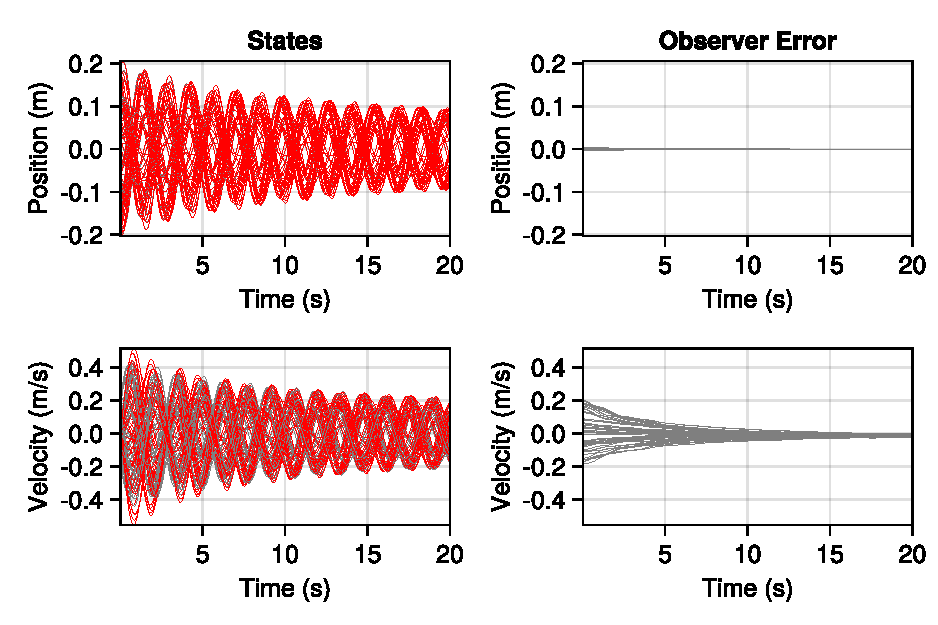
\includegraphics[width=0.47\textwidth]{Images/ren_box_obsv.pdf}
    \caption{Simulation results showing the observer predictions and observer error with the box starting at 50 different initial conditions. The left panels compare the true (grey) and estimated (red) states, while the right panels show the observer error $x - \hat{x}$ over time. The observer error converges for all 50 test cases.}
    \label{fig:observer-results}
\end{figure}

The results are plotted in Figure \ref{fig:observer-results}. In the left-hand panels, the observer predictions (red) almost exactly match the true states (grey) after approximately 4\,s. This is confirmed by the right-hand panels, which show the observer error $x_t - \hat{x}_t$ smoothly converging to zero as the observer estimates the correct states for all simulations. 

It is worth noting that at no point did we directly train the REN to minimise the observer error. This is a natural result of using a model that is guaranteed to be contracting, and training it to minimise the one-step-ahead prediction error. There is still some residual observer error in the velocity in Figure \ref{fig:observer-results}, since our observer was only trained to approximately satisfy the correctness condition. However, this could easily be reduced or eliminated using a larger observer model, more training data, and more training epochs.